\section{Các tính năng chính}
\subsection{Panels}
Grafana cung cấp các bảng biểu, đồ thị đa dạng bao gồm bản đồ nhiệt, histograms, đồ thị, biểu đồ địa lý để trực quan hoá dữ liệu một cách linh động theo bất kì cách nào chúng ta muốn.
\begin{figure}[H] % places figure environment here   
    \centering % Centers Graphic
    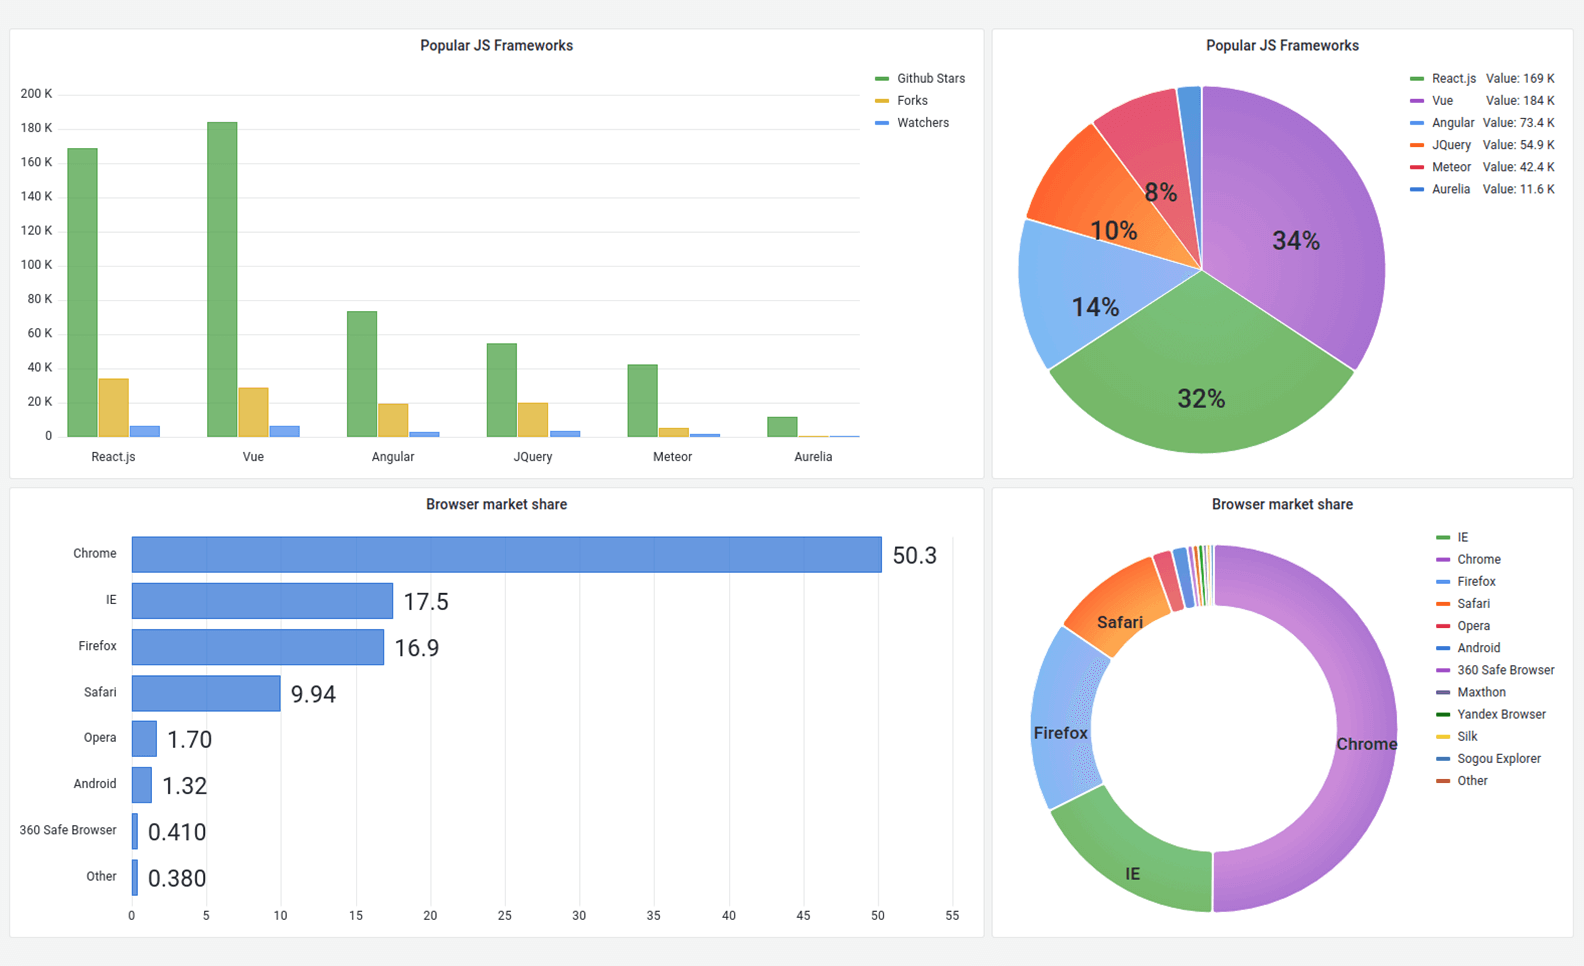
\includegraphics[width=0.8\textwidth]{figures/bar_chart_and_pie_chart_light_theme_sized.png} 
    \caption{Biểu đồ cột và biểu đồ tròn} % Creates caption underneath graph
    \label{fig:fig_01}
\end{figure}
\begin{figure}[H] % places figure environment here   
    \centering % Centers Graphic
    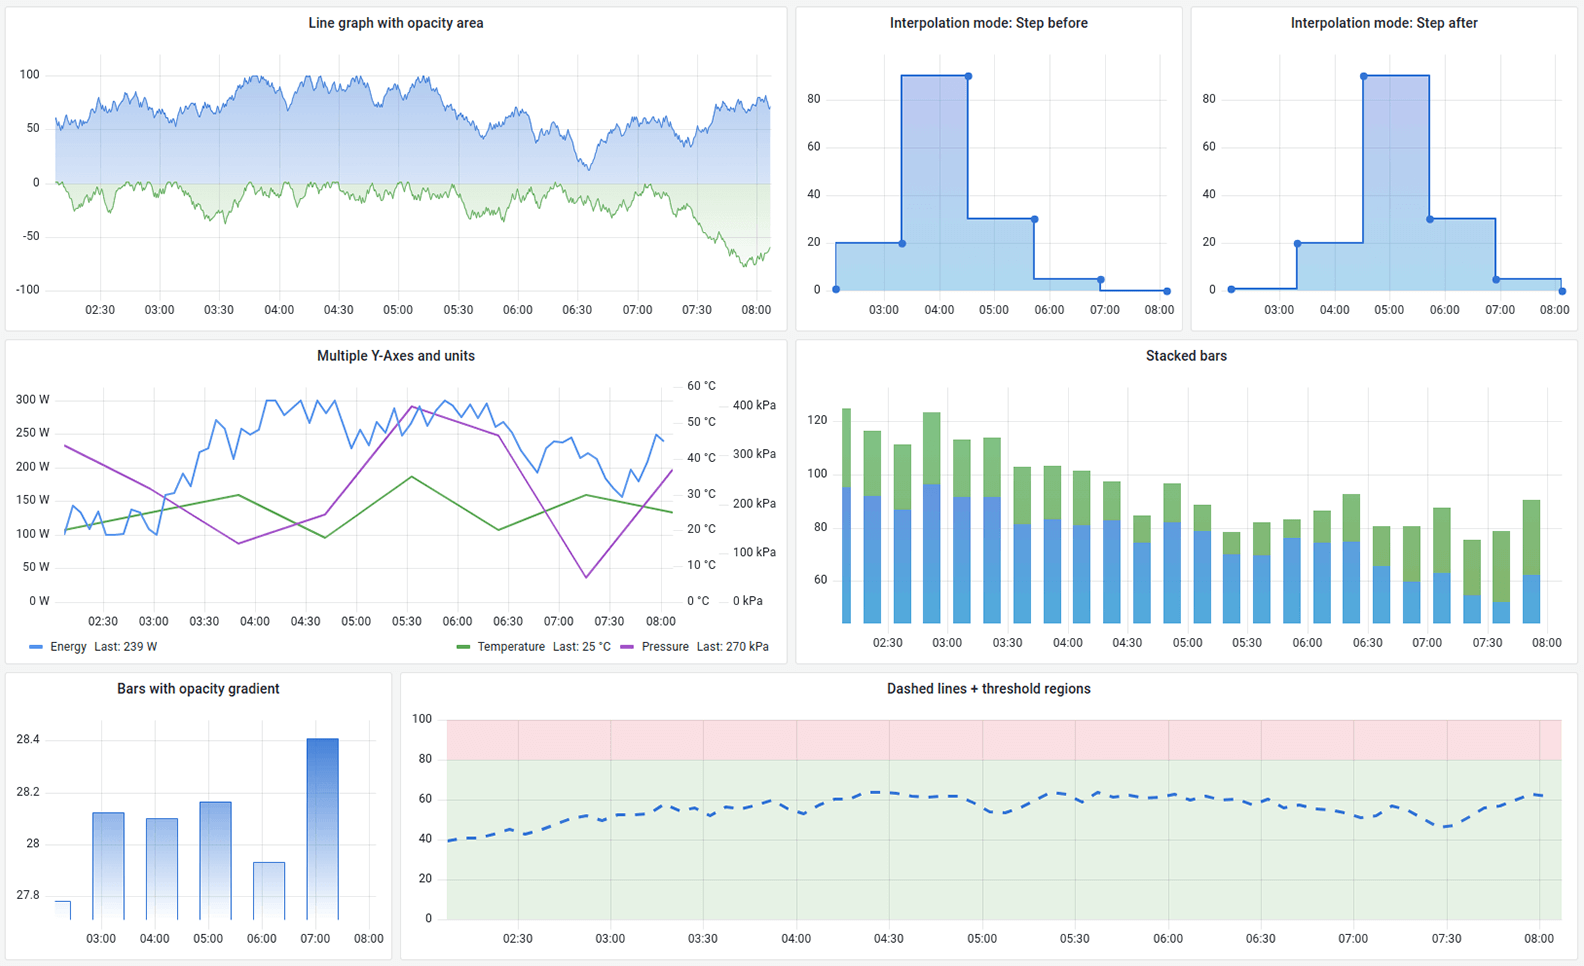
\includegraphics[width=0.8\textwidth]{figures/time_series_light_theme_sized.png} 
    \caption{Biểu đồ dữ liệu hướng thời gian} % Creates caption underneath graph
    \label{fig:fig_01}
\end{figure}
\begin{figure}[H] % places figure environment here   
    \centering % Centers Graphic
    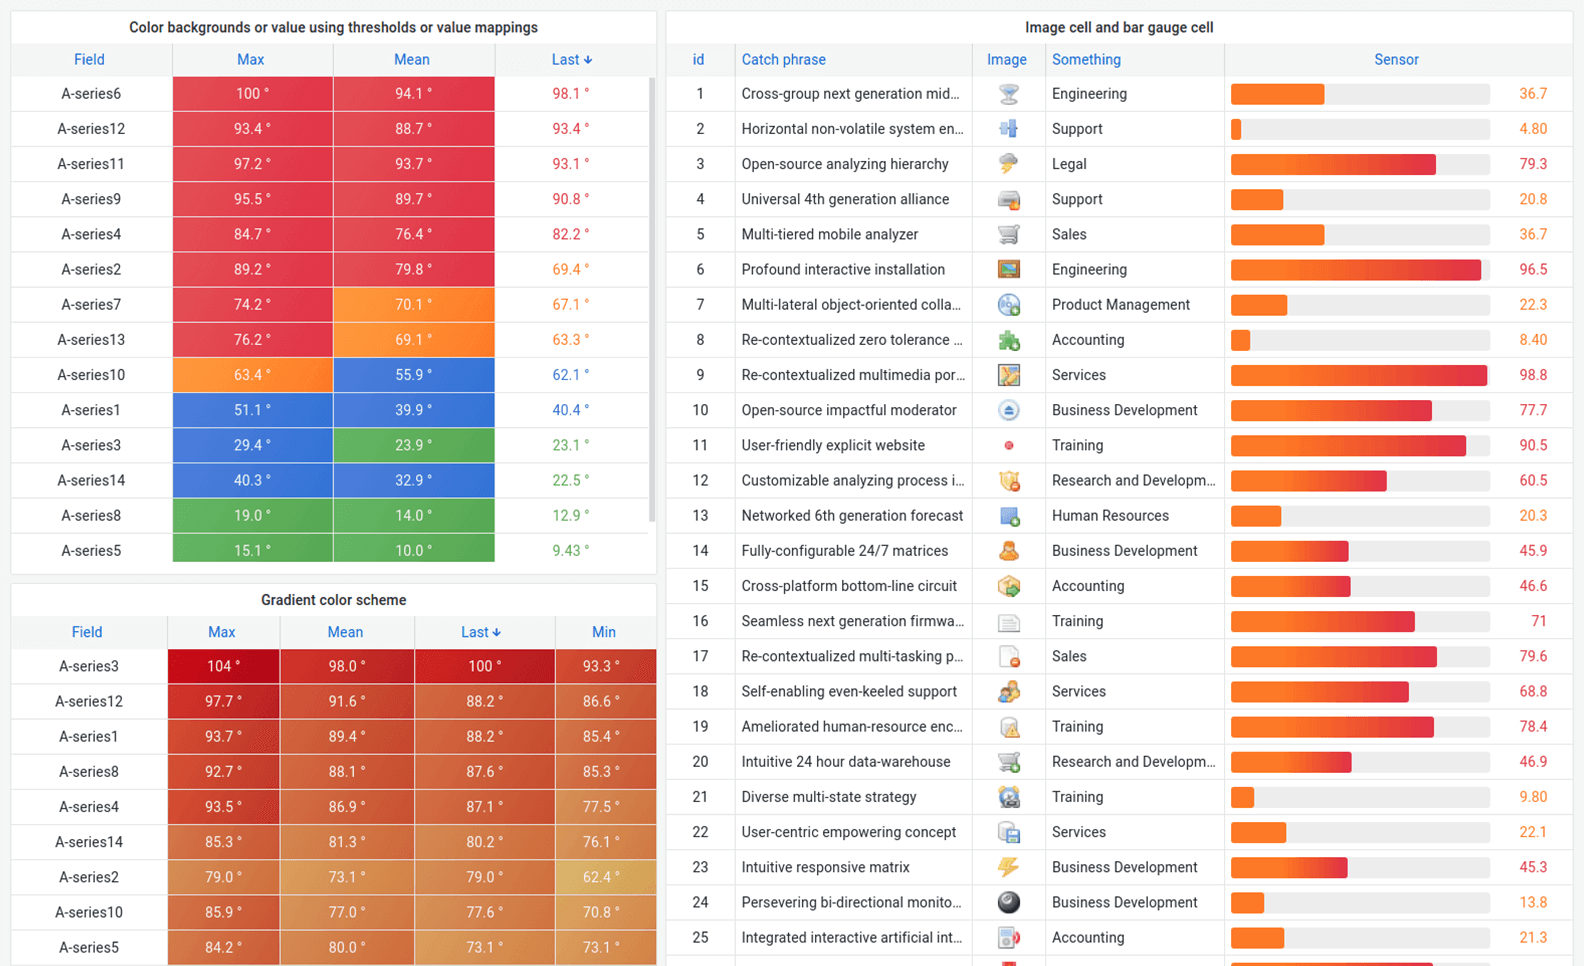
\includegraphics[width=0.8\textwidth]{figures/table_light_theme_sized.png} 
    \caption{Biểu dữ liệu dạng bảng} % Creates caption underneath graph
    \label{fig:fig_01}
\end{figure}
\begin{figure}[H] % places figure environment here   
    \centering % Centers Graphic
    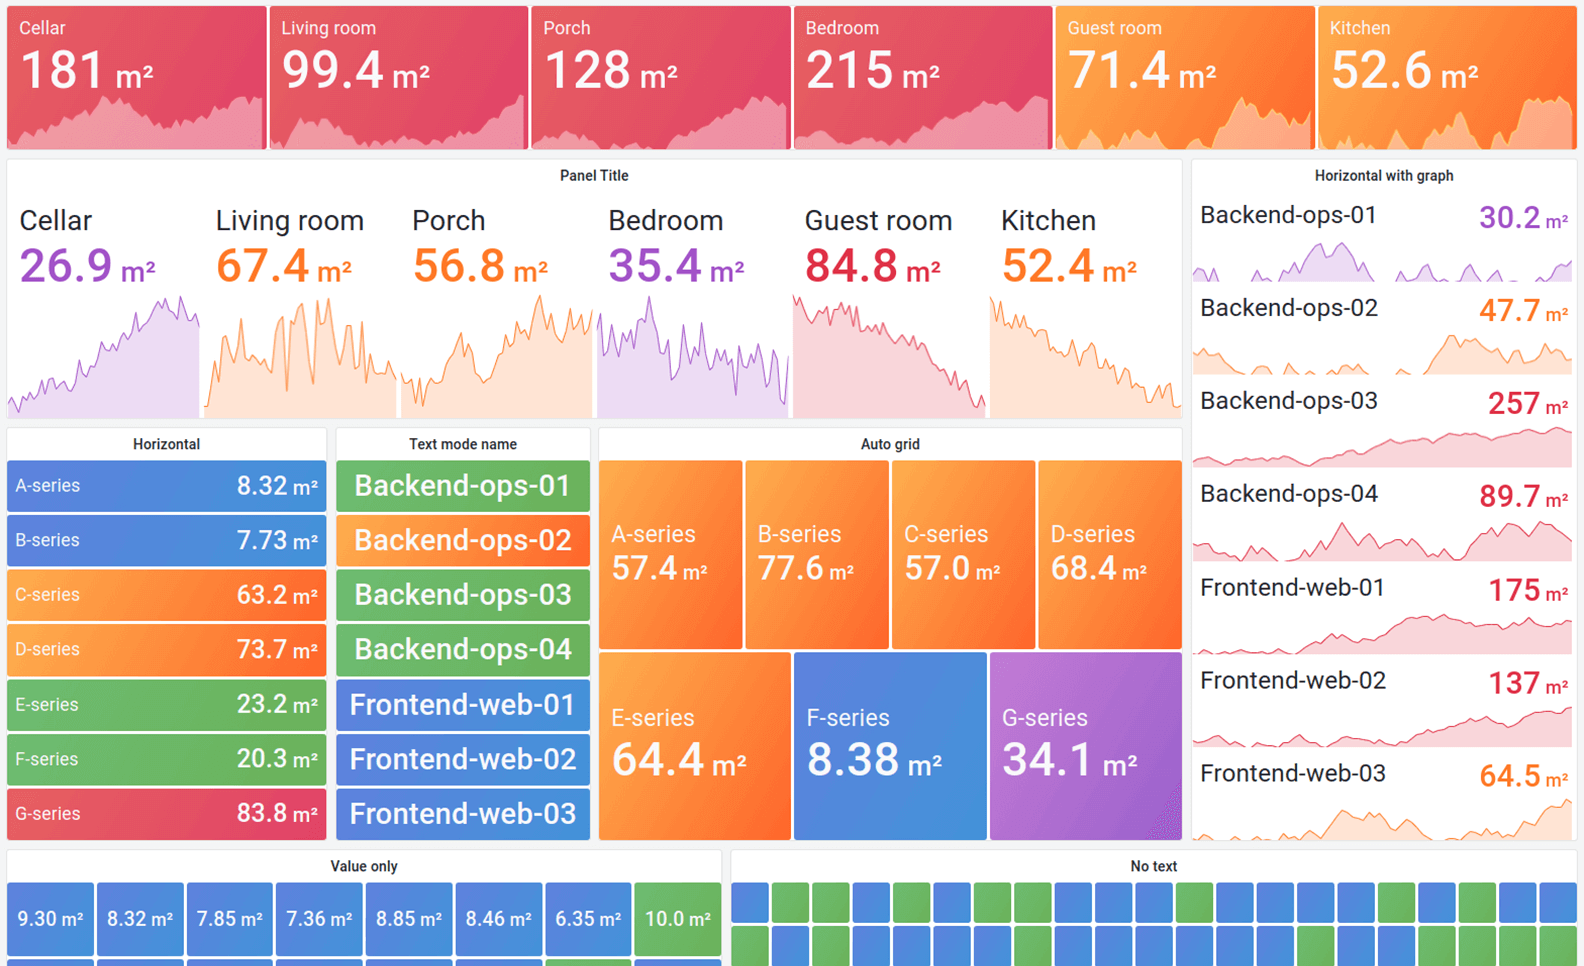
\includegraphics[width=0.8\textwidth]{figures/stat_light_theme_sized.png} 
    \caption{Biểu đồ thống kê} % Creates caption underneath graph
    \label{fig:fig_01}
\end{figure}

\subsection{Plugins}
\begin{figure}[H] % places figure environment here   
    \centering % Centers Graphic
    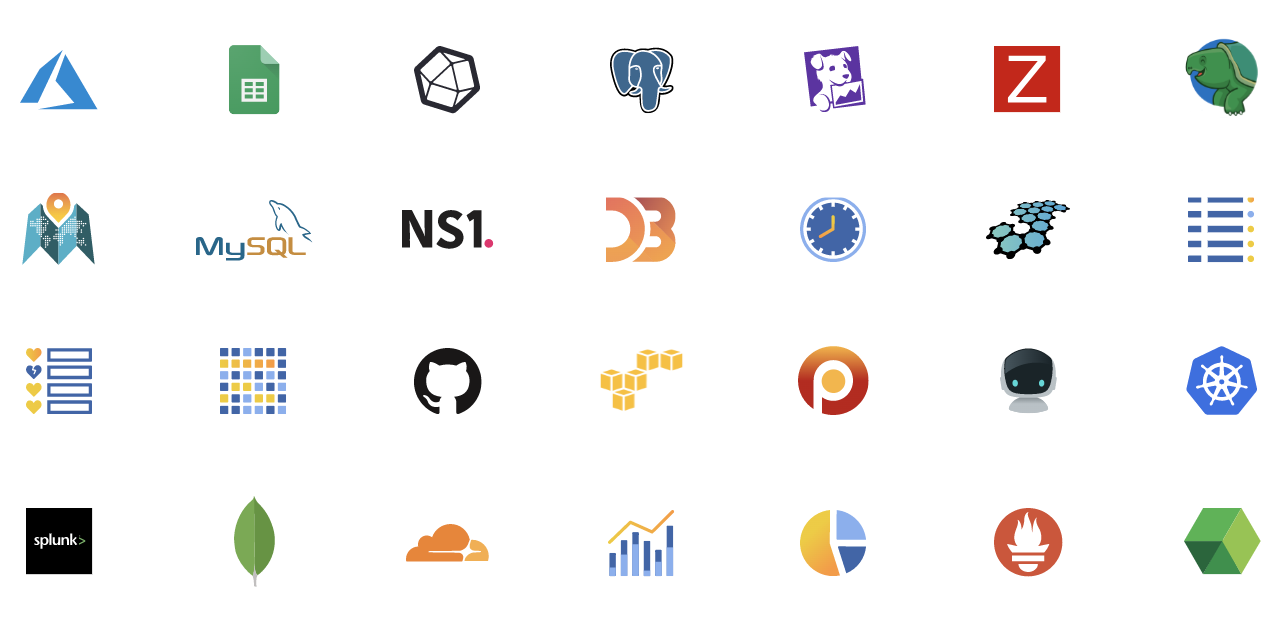
\includegraphics[width=0.8\textwidth]{figures/grafana_plugins.png} 
    \caption{Các tiện ích mở rộng} % Creates caption underneath graph
    \label{fig:fig_01}
\end{figure}
Grafana không yêu cầu phải lưu dữ liệu vào một cơ sở dữ liệu tập trung, thay vào đó nó cung cấp các tiện ích mở rộng cho phép ta kết nối tới nhiều loại cơ sở dữ liệu khách nhau. Ngoài ra Grafana cũng cho phép kết nối tới các công cụ nội bộ, cho phép doanh nghiệp triển khai một cách độc lập mà không cần phải thông qua một bên thứ ba nữa. Ví dụ chúng ta có thể phân quyền người dùng với hệ thống xác thực tập trung riêng của doanh nghiệp hoặc cũng có thể tuỳ chỉnh hệ thống cảnh báo để gửi tin về hệ thống nhắn tin riêng mà không cần thông qua những hệ thống chung như email.

\subsection{Cảnh báo (Alerting)}
\begin{figure}[H] % places figure environment here   
    \centering % Centers Graphic
    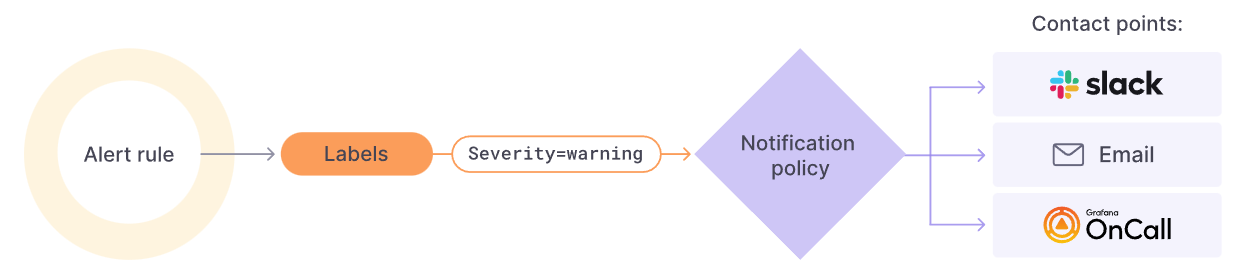
\includegraphics[width=0.8\textwidth]{figures/Alerting.png} 
    \caption{Grafana Alerting} % Creates caption underneath graph
    \label{fig:fig_01}
\end{figure}
Chức năng cảnh báo của Grafana cho phép bạn kiểm soát cho các chỉ báo đo lường và nhật ký phần mềm trong ngưỡng cho phép, bất kể chúng được lưu trữ ở đâu. Bạn có thể nhanh chóng khởi tạo, quản lý hệ thống cảnh báo chỉ trong một cửa sổ tích hợp duy nhất dù cho dữ liệu có thể đến từ nhiều nguồn khác nhau, giúp cho việc nhận dạng và giải quyết lỗi trở nên dễ dàng và thuận tiện hơn rất nhiều. Bên cạnh đó, đính kèm theo các thông báo Grafana còn cung cấp các biểu đồ, hình ảnh giúp chúng ta có thể nhanh chóng thu hẹp, khoanh vùng vấn đề đang xảy ra. Hình ảnh ở trên mô tả cách thức hoạt động của hệ thống cảnh báo Grafana. Trong đó:
\begin{itemize}
    \item \textit{Labels (nhãn)} kết nối các trường hợp cần đưa ra cảnh báo với chế độ thông báo (notification policy) tương ứng. Các lables cũng có thể được sử dụng để nhóm các cảnh báo theo mức độ nghiêm trọng của chúng.
    \item \textit{Notification policy (chế độ thông báo)} là một chuỗi các quy tắc trong đó xác định địa điểm, thời gian và cách thức mà các cảnh báo được gửi đi. Các chế độ thông báo được lập thành một kiến trúc hình cây, trong đó mỗi chế độ được gán cho một nhãn cảnh báo cụ thể. 
    \item \textit{Contact points (điểm tương tác)} xác định các đầu mối sẽ được thông báo khi xuất hiện cảnh báo. Grafana hỗ trợ nhiều công cụ liên lạc khác nhau để đảm bảo thông báo chắc chắn sẽ được gửi tới người nhận.
\end{itemize}
\begin{figure}[H] % places figure environment here   
    \centering % Centers Graphic
    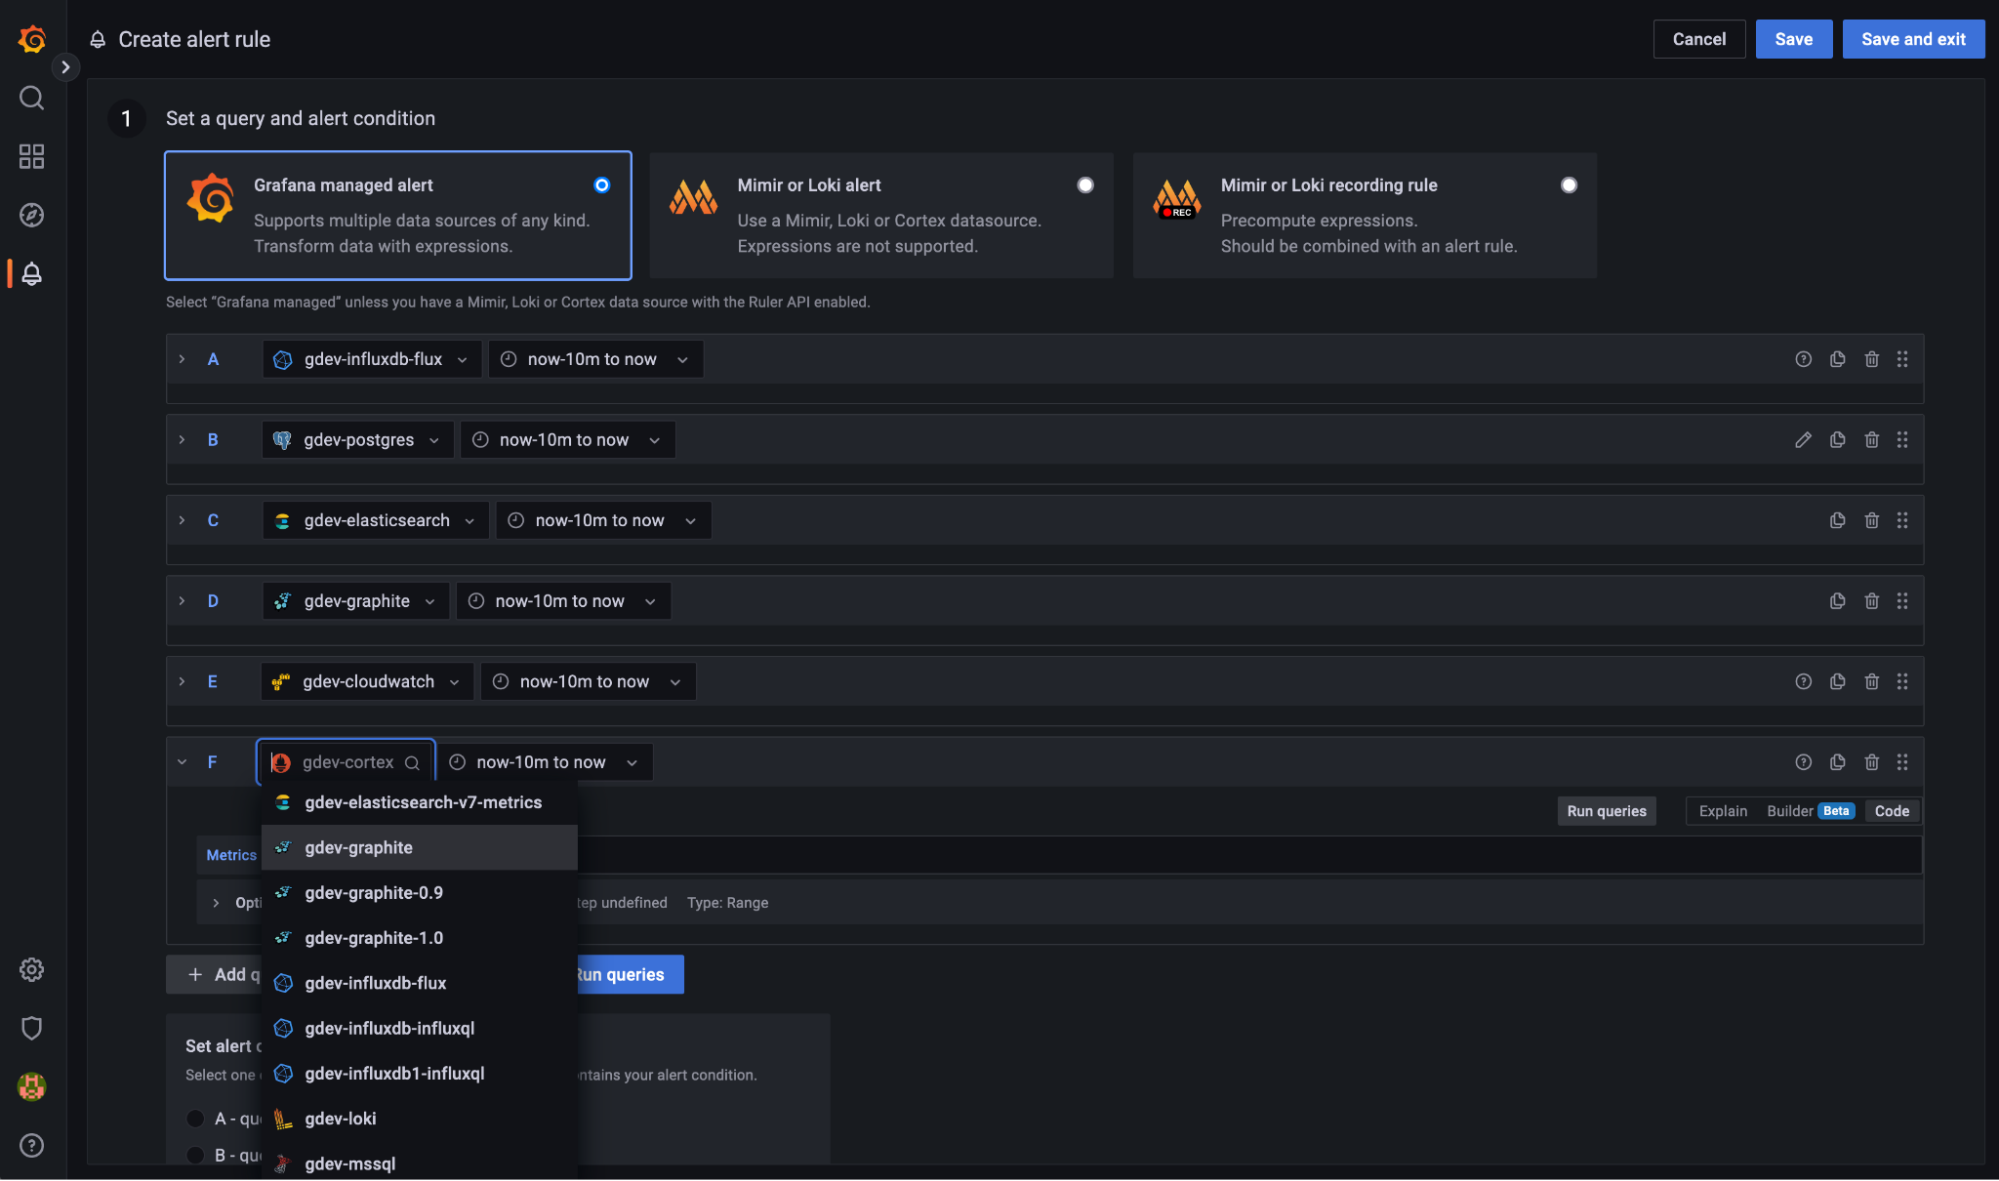
\includegraphics[width=1\textwidth]{figures/grafana-alerting-multiple-data-sources.png} 
    \caption{Cài đặt tất cả cảnh báo trong một cửa sổ duy nhất với dữ liệu từ nhiều nguồn khác nhau} % Creates caption underneath graph
    \label{fig:fig_01}
\end{figure}
\begin{figure}[H] % places figure environment here   
    \centering % Centers Graphic
    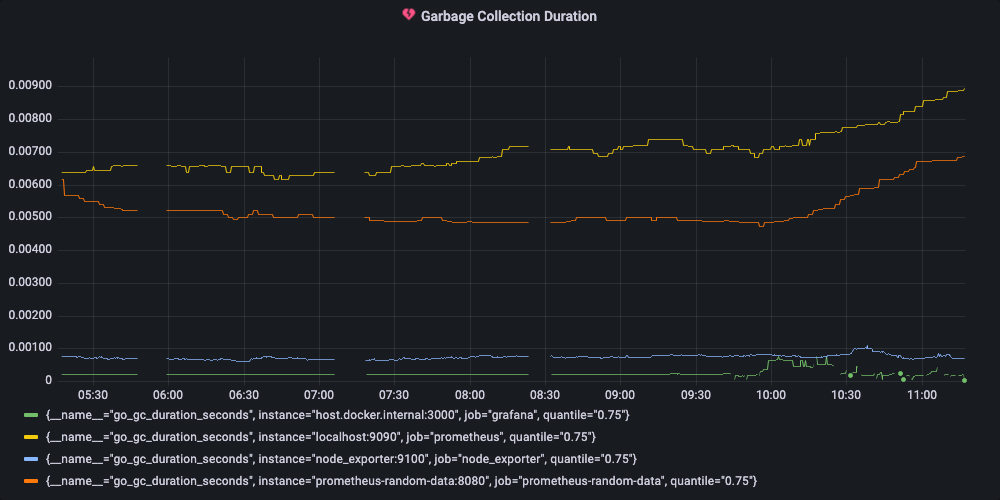
\includegraphics[width=1\textwidth]{figures/grafana-alerting-images-in-notifications.png} 
    \caption{Hình ảnh được đính kèm trong thông báo} % Creates caption underneath graph
    \label{fig:fig_01}
\end{figure}
